\documentclass[12pt,openany]{book}      
% paper size is in options.sty
\usepackage[utf8x]{inputenc}
\usepackage[colorlinks=true,citecolor=black,urlcolor=darkgray,linkcolor=black]{hyperref}
\usepackage{svg} % automatically convert svg and include
\usepackage{graphicx}
\usepackage[UKenglish]{babel}
\usepackage[T1]{fontenc}
\usepackage{amsmath,amssymb,amsthm}
\usepackage[type={CC},modifier={by-sa},version={4.0}]{doclicense}
\usepackage[skins,breakable,theorems]{tcolorbox}
\usepackage{enumitem} % spacing for lists
\setlist{noitemsep,topsep=2pt}
\usepackage{pgfplots} \pgfplotsset{compat=1.10} % also includes tikz
\usepgfplotslibrary{fillbetween}
% \usetikzlibrary{external} % To speed up compile
% \tikzexternalize[prefix=figures/]


\usetikzlibrary{positioning, arrows.meta}

%%%%%%%%%%%%%%% Arrow to position in vector
\newcommand{\here}[2]{\tikz[remember picture]{\node[inner sep=0](#2){#1}}}
%%%%%%%%%%%%%%%%%%%


\usepackage{varwidth}


%%%%%%%%%% BOOK INFORMATION %%%%%%%%%%
\newcommand{\authorname}{Everyone who contributed.}
\newcommand{\booktitle}{Mathematical Analysis 2}
\newcommand{\subtitle}{Lecture notes 2021/22}
\newcommand{\publisher}{\texttt{github.com/oliver-butterley/ma2}}
\newcommand{\editionyear}{2021}
\title{\booktitle}
\author{\authorname}
    
\theoremstyle{plain}
\newtheorem{theorem}{Theorem}
\newtheorem*{theorem*}{Theorem}
\newtheorem{lemma}{Lemma}
\theoremstyle{definition}
\newtheorem{example}{Example}
\newtheorem*{example*}{Example}
\newtheorem{definition}{Definition}
\theoremstyle{remark}
\newtheorem{remark}{Remark}

% Highlighted versions of definition and theorem
\tcolorboxenvironment{definition}{
    colback=blue!5!white, 
    arc=2mm,  enhanced, frame hidden, oversize,
    left=2mm,right=2mm,top=1mm,bottom=1mm}
\tcolorboxenvironment{theorem}{
    colback=blue!5!white, 
    arc=2mm,  enhanced, frame hidden, oversize,
    left=2mm,right=2mm,top=1mm,bottom=1mm}

    
    \colorlet{paleBlue}{blue!10!white}

\usepackage{misc/options}

%%%%%%%%% helpers
\newcommand{\abs}[1]{\left|#1\right|}
\newcommand{\bC}{\mathbb{C}} % Complex numbers
\newcommand{\bN}{\mathbb{N}} % Natural numbers
\newcommand{\bR}{\mathbb{R}} % Real numbers
%%%%%%%%%

\newcommand{\norm}[1]{\left\|#1\right\|} % Norm
\renewcommand{\aa}{\mathbf{a}}
\newcommand{\bb}{\mathbf{b}}
\newcommand{\cc}{\mathbf{c}}
\newcommand{\ee}{\mathbf{e}}
\newcommand{\ff}{\mathbf{f}}
\renewcommand{\gg}{\mathbf{g}}
\newcommand{\hh}{\mathbf{h}}
\newcommand{\rr}{\mathbf{r}}
\newcommand{\uu}{\mathbf{u}}
\newcommand{\vv}{\mathbf{v}}
\newcommand{\ww}{\mathbf{w}}
\newcommand{\xx}{\mathbf{x}}
\newcommand{\yy}{\mathbf{y}}
\newcommand{\zz}{\mathbf{z}}
\newcommand{\aalpha}{\boldsymbol{\alpha}}


\begin{document}

% Reduce space around displayed equations
\setlength{\abovedisplayskip}{10pt}
\setlength{\belowdisplayskip}{10pt}

\frontmatter
\pagestyle{empty}

% Half title page
% {
% 	\centering

% 	~

% 	\vspace{24pt}
% 	{\scshape\Huge \booktitle \par}
% }

% Title page
\begin{titlepage}
	\centering

	~

	\vspace{24pt}
	{\scshape\Huge \booktitle\par}
	\vspace{6pt}
	{\scshape\large \subtitle\par}
	\vspace{\stretch{1.25}}
	{\itshape\large by\par}
	\vspace{6pt}
	{\itshape\Large \authorname\par}
	\vspace{\stretch{6}}
	{\large \publisher\par}
\end{titlepage}

% Copyright page

{\small
\setlength{\parindent}{0em}\setlength{\parskip}{1em}

~

\vfill


\doclicenseIcon
This text is licensed under 
\doclicenseLongNameRef \ 
(\doclicenseNameRef).

You are free to 
\textbf{share} this work (copy and redistribute the material in any medium or format) 
and 
\textbf{adapt} this work (remix, transform, and build upon the material for any purpose, even commercially),
under the obligation of 
\textbf{attribution} (you must give appropriate credit)
and
\textbf{share alike} (if you remix, transform, or build upon the material, you must distribute your contributions under the same license as the original). 

This text may contain errors, inaccuracies and misleading ideas, the reader takes full responsibility for the consequences. 
Any resemblance to actual persons, living or dead, events or localities is entirely coincidental.

Typeset: \today

Source available at: \publisher{}
}

\chapter{Preface}
\lettrine{T}{his} text accompanies the course ``Mathematical Analysis 2'' taught at the University of Rome Tor Vergata in the department of engineering 2022--2025.
During these years the course was led by Oliver Butterley. 

The aim of this document is to concisely describe the fundamental details related to the material of the course.
They are aptly named as ``notes'' and are most likely not the comprehensive source of all relevant information.
We have easy access to a huge volume of resources and so here we will make connections to whatever is useful, whenever we can. 

These notes are merely written text whereas the central part of the course remains the time spent working with the material, be it doing exercises, discussing, doing calculations, etc. This is not text for memorising, this is text that aims to help us practice and become stronger thinkers.

This text is freely\footnote{Free both in the sense of \href{https://en.wikipedia.org/wiki/Gratis_versus_libre}{``free speech'' and ``free beer''}.} available at \href{https://github.com/oliver-butterley/ma2}{\textbf{github.com/oliver-butterley/ma2}}.
Everyone is encouraged to contribute improvements to the document during the progress of the course. 

Some of the text comes from previous years and from many other sources, some of the text came to be during the course.
The current version is the product of many people, in particular everyone who has made suggestions in class and pointed out errors or imprecisions and to everyone who suggested useful additional content.


% \cleardoublepage   
% % Make sure contents page starts on right-side page
\tableofcontents\thispagestyle{empty}\cleardoublepage%

\pagestyle{fancy}

\chapter{Introduction}

\lettrine{W}{e} start by looking at examples which demonstrate some of the motives behind studying analysis in general.
%
\begin{example*}[Series]
  The geometric series
  \(S = 1 + \frac{1}{2} + \frac{1}{4} + \frac{1}{8} + \frac{1}{16} + \cdots\)
  can be summed by the following simple simple trick.
  Multiplying by \(2\) we obtain that
  \[
    2S = 2 + 1 + \frac{1}{2} + \frac{1}{4} + \frac{1}{8} + \frac{1}{16} + \cdots = 2+S
  \]
  and so \(S=2\).
  If we try to do the same to the sum
  \(T = 1 + 2 + 4 + 8 + 16 + \cdots\)
  we get the nonsensical answer
  \[
    2T = 2 + 4 + 8 + 16 + \cdots = T -1
  \]
  and so \(T = -1\).
  %
  Why should we trust the argument in the first case and not in the second?
\end{example*}


\begin{example*}[Interchanging sums]
  If we consider any matrix of numbers, for example,
  \[
    \begin{pmatrix}
      1 & 2 & 3 \\
      4 & 5 & 6 \\
      7 & 8 & 9
    \end{pmatrix}
  \]
  we can sum first the rows \(6 + 15 + 24 = 45\) or first the columns \(12 + 15 + 18 = 45\) to obtain the total sum of all numbers.
  This is the rule
  \[
    \sum_{j=1}^{m} \sum_{k=1}^{n} a_{jk} = \sum_{k=1}^{n} \sum_{j=1}^{m}  a_{jk}.
  \]
  We would like to believe that also \(\sum_{j=1}^{\infty} \sum_{k=1}^{\infty} a_{jk} = \sum_{k=1}^{\infty} \sum_{j=1}^{\infty}  a_{jk}\).
  However this doesn't work for the following matrix:
  \[
    \begin{pmatrix}
      1      & 0      & 0      & \cdots \\
      -1     & 1      & 0      & \cdots \\
      0      & -1     & 1      & \cdots \\
      \vdots & \vdots & \vdots & \ddots
    \end{pmatrix}
  \]
  %
  We often want to swap the order of summing (or integrating) and often need to consider infinite sums (or integrals).
  When can we do this and can't we?
\end{example*}

\begin{example*}[Interchanging integrals]
  Let's try to integrate \(e^{-xy} - xye^{-xy}\) with respect to both \(x\) and \(y\).
  We would like to believe that
  \[
    \int_{0}^{\infty} \int_{0}^{1} (e^{-xy} - xye^{-xy}) \ dy \ dx
    \overset{\text{\large\color{blue} ?}}{=} \int_{0}^{1} \int_{0}^{\infty}  (e^{-xy} - xye^{-xy}) \ dx \ dy.
  \]
  Since
  \( \int_{0}^{1} (e^{-xy} - xye^{-xy}) \ dy = \left[ ye^{-xy} \right]_{y=0}^{1} = e^{-x}\),
  the left-hand side is
  \( \int_{0}^{\infty} e^{-x} \ dx = \left[ -e^{-x} \right]_{0}^{\infty} = 1 \).
  However, since
  \( \int_{0}^{\infty}  (e^{-xy} - xye^{-xy}) \ dx = \left[ xe^{-xy} \right]_{x=0}^{\infty} = 0\),
  the right-hand side is \(\int_{0}^{1} 0 \ dx = 0\).
  So how do we know when to trust the interchange of intervals?
\end{example*}


\begin{example*}[interchanging limits]
  We could easily believe that
  \[
    \lim_{x\to 0}\lim_{y\to 0} \frac{x^2}{x^2 + y^2}
    \overset{\text{\large\color{blue} ?}}{=}
    \lim_{y\to 0}\lim_{x\to 0} \frac{x^2}{x^2 + y^2}.
  \]
  However \(\lim_{y\to 0} \frac{x^2}{x^2 + y^2} = \frac{x^2}{x^2 + 0} = 1 \) and so the left-hand side is \(1\)
  whereas \(\lim_{x\to 0} \frac{x^2}{x^2 + y^2} = \frac{0}{0 + y^2} = 0\) so the right-hand side is \(0\).
  This example shows that the interchange of limits is untrustworthy. Under what circumstances is it legitimate?
\end{example*}

We need to be rigorous in our logic otherwise, as we have seen in these examples, the conclusions can be erroneous and the difficulties are often subtle.

\subsection*{Curves of constant width}
%
\begin{figure}[htb]
  \centering
  \includesvg[width=0.6\textwidth]{reuleaux.svg}
  \caption{The Reuleaux triangle is a curve of constant width.}
  \label{fig:reuleaux}
\end{figure}
%
The above examples are calculus based but it is worthwhile to consider a real world application of the rigour and reasoning we aspire to.
Suppose we are organising the production facilities which manufacture a component that is round (maybe a rocket body, maybe a tube, etc.).
\begin{samepage}
  As part of the production it is important to have a procedure which guarantees that the fabrication is done to the correct tolerance.
  The idea proposed is:
  \begin{quotation}
    ``We measure the width from all angles to confirm that the manufactured component is correct.''
  \end{quotation}
\end{samepage}
Two-dimensional problem in the sense we assume that the object is a closed curve in \(\bR^2\).
For a given angle we define the width of this curve to be the smallest distance between two parallel lines which touch the curve in a single point but never cross it (one each side of the curve).
We say that the curve has constant width if this width is equal from every direction.
This is just what we would check using calipers on a part and rotating.
The following statement is intuitive and true.
\begin{theorem*}
  A circle has constant width.
\end{theorem*}
\noindent
However the converse is not true, indeed the following is true.
\begin{theorem*}
  There exist constant width curves which are not circles.
\end{theorem*}
\noindent
This can be proved by constructing many such curves, for example the \href{https://en.wikipedia.org/wiki/Reuleaux_triangle}{Reuleaux triangle}. Indeed there are such curves which look similar to regular polygons but still have constant width.


% \footnotetext{
%   Source of Figure~\ref{fig:reuleaux}: 
%   \url{https://commons.wikimedia.org/wiki/File:Reuleaux_supporting_lines.svg}
%   }



\subsection*{MA2 versus MA1}

Much of what we do in this course builds on ideas established in Mathematical Analysis 1.
In particular many of the ideas are extended to the higher dimensional setting.

\begin{center}
  \begin{tabular}{r | l}
    \textbf{Mathematical Analysis 1}
     &
    \textbf{Mathematical Analysis 2}  \\
    \hline
    Sequences \& series of numbers
     &
    Sequences \& series  of functions \\
    \(a_1, a_2, a_3,\ldots \)
     &
    \(f_1(x), f_2(x), f_3(x),\ldots \)
    \\
    \(\sum_{j=0}^{\infty} a_j\)
     &
    \(\sum_{j=0}^{\infty} f_j(x)\)
    \\
    \hline
    (Functions) \(f:\bR \to \bR\)
     &
    \(f:\bR^n \to \bR\) (Scalar fields)
    \\
     &
    \(\mathbf{f}:\bR^n \to \bR^n\) (Vector fields)
    \\
     &
    \(\boldsymbol{\alpha}:\bR \to \bR^n\) (Paths)
    \\
    \hline
    (Derivative) \( f'(x) = \frac{df}{dx}(x)\)
     &
    \( \frac{\partial f}{\partial x_j}(x_1,\ldots,x_n)\) (Partial derivatives)
    \\
     &
    \(\nabla f\) (Gradient)
    \\
     &
    \(D_v f\) (Directional derivative)
    \\
     &
    \(\boldsymbol{\alpha}'\) (Derivative of path)
    \\
     &
    \(Df\) (Jacobian matrix)
    \\
    \hline
    (Extrema) \(\sup_{x\in \bR} f(x)\)
     &
    \(\sup_{x\in \bR^n} f(x)\) (Extrema)
    \\
     &
    Lagrange multiplier method
    \\
    \hline
    Integral \(\int_{a}^{b} f(x) \ dx\)
     &
    Multiple integral
    \\
     &
    Line integral
    \\
     &
    Surface integral
  \end{tabular}
\end{center}


\subsection*{Suggested further reading}

\begin{itemize}
  \item "Analysis 1" by Terence Tao.
        (Particularly \S 1.2 ``Why Analysis?'' and Appendix A ``The basics of mathematical logic'').
\end{itemize}

\mainmatter


\chapter{Sequences and series of functions}

\lettrine{A}{nalogously} to sequences of numbers we can consider a sequence of functions \(f_0(x),f_1(x), f_2(x), f_3(x),\) etc.
Often it is convenient to write such a sequence as \(\{ f_n(x)\}_{n\in \mathbb{N}}\).
For example, the following are sequences of functions.
\begin{itemize}
  \item \(f_1(x) = x^2, f_2(x)=x^4, f_3(x)=x^6,\ldots \)
  \item \(f_1(x) = e^x, f_2(x)=e^{2x}, f_3(x)=e^{3x},\ldots \)
  \item \(f_n(x) = n \exp \left( - \frac{1}{2}n^2 x^2 \right)\)
\end{itemize}

Note that in the first case we could have instead written \(f_n(x) = x^{2n}\) and in the second case we could have written  \(f_n(x) = e^{nx}\).
The natural number \(n\) is called the index.
Typically the index of the sequence starts from \(n=0\) or \(n=1\) but that's not essential.
The index doesn't need to be \(n\), any other letter, or indeed symbol, can be used.


\section{Convergence and continuity}

We start by recalling the notion of convergence for sequences of numbers.

\begin{definition}
  A sequence of numbers  \(a_1, a_2, a_3,\ldots \) is said to \emph{converge} to \(a\) if, for each \(\epsilon>0\), exists \(N\in \mathbb{N}\) such that \(|a_n - a| < \epsilon\) whenever \(n\geq N\).
\end{definition}
%
\noindent
If a sequence \({\{a_n\}}_{n}\) converges to \(a\) then we write \(a_n \to a\) (as \(n\to \infty\)).
For sequences of functions we will need to consider two different notions of convergence.
In order to understand this difficulty let us consider the following example.

\begin{example*}
  Consider the sequence \(f_n(x) = x^n\) for \(x\in (0,1)\).
  For each \(x\in (0,1)\) we see that \(f_n(x) \to 0\).
  On the other hand, for each \(n\), \(2^{\frac{1}{n}}\in (0,1)\) and \(f_n(2^{\frac{1}{n}}) = \frac{1}{2}\).
\end{example*}


\begin{figure}
  \begin{center}
    \includegraphics{sequence-xn.pdf}
    \caption{The sequence of functions \(f_n(x)= x^n\).}
  \end{center}
\end{figure}

\noindent
Up until now we haven't mentioned the domain of the functions in the sequence but to proceed we need to be make this detail rigorous.
We will write that ``\({\{f_n(x)\}}_{n}\) is a sequence of functions on \(D\subset \bR\)'' to mean that there is a fixed \(D\subset \bR\) and, for each \(n\in \bN\), \(f_{n}\) is a function with domain \(D\) (i.e., \(f_n : D \to \bR\)).


\begin{definition}[pointwise convergence]
  Let \(D\subset \mathbb{R}\),
  let \(f_n(x)\) be a sequence of functions on \(D\)
  and let \(f(x)\) be a function on \(D\).
  If \(f_n(x) \to f(x)\) for each \(x\in D\) we say that \(f_n\) is \emph{pointwise convergent} to \(f\).
\end{definition}

\begin{definition}[uniform convergence]
  Let \(f_n(x)\) be a sequence of functions on \(D\subset \mathbb{R}\)
  and let \(f(x)\) be a function on \(D\).
  If, for each \(\epsilon>0\), there exists \(N\) such that for every \(n\geq N\) and every \(x\in D\), \(|f_n(x) - f(x)| < \epsilon\) then we say that \(f_n\) is \emph{uniformly convergent} to \(f\).
\end{definition}

\noindent
\textbf{Problem:}
Show that the sequence \(f_n(x) = x^n\) converges uniformly on \((0,\frac{1}{2})\).

\noindent
\textbf{Solution:}
We observe that it converges pointwise to the constant function \(f(x)=0\).
\begin{itemize}
  \item We also observe that \(|f_n(x) - f(x) | \leq \frac{1}{2^n}\) for all \(x\in (0,\frac{1}{2})\).
  \item This means that, for every \(\epsilon>0\), if we can choose \(N=-\log_{2}\epsilon\) then \(|f_n(x) - f(x) | \leq \epsilon\) whenever \(n\geq N\).
\end{itemize}


\begin{definition}
  Let \(f(x)\) be a functions on \(D\subset \mathbb{R}\).
  We say that \(f\) is \emph{continuous} at \(p\in D\) if, for each \(\epsilon>0\), there is \(\delta >0\) such that \(|f(x)-f(p)| <\epsilon\) whenever \(x\in D\), \(|x-p| <\delta\).
  We say that \(f\) is \emph{continuous on \( D\)} if \(f\) is continuous at every \(p\in D\).
\end{definition}




\begin{figure}
  \begin{center}
    \includegraphics{sequence-arctan.pdf}
    \caption{The sequence of functions \(f_n(x)= \arctan(nx)\).}
  \end{center}
\end{figure}

It is natural to consider a sequence of continuous functions which converge and ask if the function they converge to is continuous.
What about the sequence of functions \(f_n(x) = \arctan (nx)\)?

\begin{theorem}
  \label{thm:continuous-limit}
  Suppose that \(f_n \to f\) uniformly on \(D\) and that the \(f_n\) are continuous on \(D\).
  Then \(f\) is continuous on \(D\).
\end{theorem}


\begin{proof}
  Let \(p\in D\).
  Uniform convergence means that, for each \(\epsilon>0\), there exists \(N\) such that for every \(n\geq N\) and every \(x\in D\), \(|f_n(x) - f(x)| < \frac{\epsilon}{3}\).
  By continuity of \(f_N(x)\) at \(x=p\), there is a \(\delta >0\) such that \(|f_N(x)-f_N(p)| < \frac{\epsilon}{3} \) whenever \(x\in D\), \(|x-p| <\delta\).
  Since
  \[
    | f(x) - f(p) | = |f(x) - f_N(x) + f_N(x) - f_N(p) + f_N(p) - f(p) | \]
  this means that, for all \(|x-p| <\delta\),
  \[
    \begin{aligned}
      | f(x) - f(p) | & \leq   |f(x) - f_N(x)| + |f_N(x) - f_N(p)| + |f_N(p) - f(p) | \\
                      & < 3 \frac{\epsilon}{3} = \epsilon.
    \end{aligned}
  \]
  This proves the continuity of \(f\) at \(p\). Since \(p\in D\) is arbitrary this shows the continuity of \(f\) on \(D\).
\end{proof}


Recall that integrals are defined rigorously using the notion of a step functions.

\begin{theorem}
  \label{thm:limit-of-integral}
  Suppose that \(f_n\) are continuous functions on \([a,b] \subset \mathbb{R}\), uniformly convergent to \(f\).
  Then
  \[
    \lim_{n\to \infty} \int_{a}^{b} f_n(x) \ dx = \int_{a}^{b} f(x) \ dx.
  \]
\end{theorem}

\begin{proof}
  The uniform convergence implies that for each \(\epsilon>0\), there exists \(N\) such that for every \(n\geq N\) and every \(x\in D\), \(|f_n(x) - f(x)| <  \frac{\epsilon}{b-a}\).
  This means that
  \[ \Big| \int_{a}^{b} f_n(x) \ dx - \int_{a}^{b} f(x) \ dx \Big|
    \leq \int_{a}^{b} | f_n(x) - f(x) | \ dx
    \leq (b-a) \frac{\epsilon}{b-a} = \epsilon.\]
  This shows that \(\int_{a}^{b} f_n(x) \ dx \to  \int_{a}^{b} f(x) \ dx\).
\end{proof}


\subsection*{Series of functions}



Recall that for a sequence \({\{a_n\}}_{n}\) of numbers,
the series \(\sum_{n}a_n\) is the sequence \({\{\sum_{k=1}^{n}a_k\}}_{n}\) of numbers (the partial sums).
We say that the series  \(\sum_{n}a_n\) is convergent if \({\{\sum_{k=1}^{n}a_k\}}_{n}\) is convergent.



\begin{definition}
  Let \(\{f_n\}\) be a sequence of functions.
  We say that the series \(\sum_{n} f_n\)
  \begin{itemize}
    \item   is \emph{pointwise convergent} if
          \(\sum_{k=1}^{n} f_k(x)\) is pointwise convergent,
    \item   is \emph{uniformly convergent} if
          \(\sum_{k=1}^{n} f_k(x)\) is uniformly convergent.
  \end{itemize}
\end{definition}


\begin{theorem}
  Suppose that the series \(\sum_{n} f_n\) is uniformly convergent to \(g\) on \(D\) and the \(f_n\) are continuous on \(D\).
  Then \(g\) is continuous on \(D\).
\end{theorem}


\begin{proof}
  If the \(f_k\) are continuous then the \(\sum_{k=1}^{n} f_k\) are continuous.
  This means that Theorem~\ref{thm:continuous-limit} applies.
\end{proof}



\begin{theorem}
  Suppose that the series \(\sum_{n} f_n\) is uniformly convergent to \(g\) and the \(f_n\) are continuous.
  Then
  \[
    \lim_{n\to\infty} \int_{a}^{b}  \sum_{k=1}^{n} f_k(x)  \ dx = \int_{a}^{b} g(x) \ dx.
  \]
\end{theorem}


\begin{proof}
  Again, that the \(f_k\) are continuous means that the \(\sum_{k=1}^{n} f_k\) are continuous.
  This means that Theorem~\ref{thm:limit-of-integral} applies.
\end{proof}


Here and subsequently it is convenient to recall three commons tests which are useful for proving convergence:
\href{https://en.wikipedia.org/wiki/Ratio_test}{ratio test},
\href{https://en.wikipedia.org/wiki/Root_test}{root test},
\href{https://en.wikipedia.org/wiki/Direct_comparison_test}{comparison test}.
%
For series of functions we have the following test for convergence.

\begin{theorem}[Weierstrass M-test]
  Suppose that \({\{f_n\}}_n\) is a sequence of functions on \(D\), that \({\{M_n\}}_n\) is a sequence of positive numbers
  and that \(|f_n(x)|\leq M_n\).
  If the series \(\sum_{n=0}^{\infty}M_n\) is convergent then the series \(\sum_{n=0}^{\infty}f_n\) is uniformly convergent.
\end{theorem}



\begin{proof}
  By the comparison test \(\sum |f_n(x)| \) is convergent for all \(x\in D\).
  I.e., for each \(x\) the series \(\sum f_n(x) \) is absolutely convergent and so we let \(f(x)\) be the limit.
  We compute
  \[
    \Big|f(x) - \sum_{k=1}^{n} f_k(x)  \Big|
    =
    \Big|\sum_{k=n+1}^{\infty} f_k(x)  \Big|
    \leq \sum_{k=n+1}^{\infty} |f_k(x)|
    \leq  \sum_{k=n+1}^{\infty} M_k.
  \]
  As \(\sum_{n}M_n\) is convergent this last expression tends to \(0\) as \(k\to \infty\).
  This estimate is independent of \(x\).
\end{proof}




\section{Power series}



\begin{definition}
  Let \({\{a_n\}}_{n}\) be a series of numbers.
  The series
  \(\sum_{n} a_n x^n\)
  is called a \emph{power series}.
\end{definition}
Typically the power series will converge for some \(x\) and diverge for other \(x\).
Note that we could permit \(x\) to be a complex number and the entire work of this section holds verbatim.
However, for the present purposes we will assume that \(x \in \bR\) and that the coefficients \(a_n \in \bR\).

\begin{example*}
  Let \(a_n = 2^{-n}\).
  The power series \(\sum_{n} a_n x^n = \sum_{n}\frac{x^n}{2^n}\) is convergent when \(\abs{x}<2\) and divergent  when \(\abs{x} > 2\).
  To see this we apply the root test and observe that  \(\lim_{n\to\infty}\big(\frac{\abs{x}^n}{2^n} \big)^{\frac{1}{n}}=\frac{\abs{x}}{2}\).
\end{example*}

\begin{example*}
  Let \(a_n = \frac{1}{n!}\).
  The power series \(\sum_{n}\frac{x^n}{n!}\) is convergent for all \(x\).
  To see this we use the ratio test and observe that  \(\abs{\frac{x^{n+1}}{(n+1)!} }/ \abs{\frac{zx^n}{n!}} = \frac{\abs{x}}{n+1}\) and that \(\lim_{n\to\infty} \frac{\abs{x}}{n+1} = 0 \) for any \(x\).
\end{example*}



\section{Radius of convergence}

A key notion is determining exactly the domain on which a power series converges.

\begin{theorem}[uniformly convergent power series]
  Suppose that \(\sum_{n}a_n x^n\) converges for some \(x=x_0 \neq 0\).
  Let \(R<\abs{x_0}\).
  Then the series is uniformly and absolutely convergent for all \(x\) such that \(\abs{x}\leq R\).
\end{theorem}

\begin{proof}
  \begin{itemize}
    \item \(\sum_n a_n x_0^n\) is convergent \(\implies\) for all \(n\), \(\abs{a_n x_0^n} \leq M\) for some \(M>0\);
    \item \(\abs{a_n x^n} = \abs{a_n x_0^n} \cdot \abs{\frac{x}{x_0}}^n \leq M \frac{R^n}{\abs{x_0}^n}\);
    \item \(\sum_n M \frac{R^n}{\abs{x_0}^n}\) is a geometric sum and so convergent;
    \item M-test \(\implies\) series is uniformly and absolutely convergent when \(\abs{x}\leq R\).  \qedhere
  \end{itemize}
\end{proof}




\begin{theorem}[radius of convergence]
  Suppose exists  \(x_1,x_2 \neq 0\) such that \(\sum_n a_n x_1^n\) is convergent and \(\sum_n a_n x_2^n\) is divergent.
  Then exists \(r>0\) such that \(\sum_n a_n x^n\) is convergent for \(\abs{x}<r\) and divergent for \(\abs{x}>r\).
\end{theorem}

\begin{proof}
  \begin{itemize}
    \item Let \(A\) be the set of real numbers for which \(\sum_n a_n x^n\) is convergent;
    \item Let \(r\) be the least upper bound of \(A\);
    \item Series  \(\sum_n a_n x^n\) is convergent whenever \(\abs{x}<r\);
    \item If \(\abs{x}>r\) and \(\sum_n a_n x^n\) is convergent then this contradicts the definition of \(A\) and so  \(\sum_n a_n x^n\) is divergent for \(\abs{x}>r\). \qedhere
  \end{itemize}
\end{proof}


\begin{definition}
  This \(r\) is called the \emph{radius of convergence} for the power series \(\sum_n a_n z^n\).
\end{definition}

We use the following convention:
if \(\sum_n a_n x^n\) converges for all \(x\in \bC\) we say the radius of convergence is \(\infty\);
if \(\sum_n a_n x^n\) doesn't converge except  \(x=0\) we say the radius of convergence is \(0\).

Note: all of the above concerning power series holds verbatim for \(x\) a complex number and so ``radius'' is more meaningful since it truly corresponds to a disk in the complex plane.




\section{Integrating and differentiating power series}



Let \(a_n \in \bR\), \(x\in \bR\).
If \(\sum_n a_n x^n\)converges we define the function \(f(x) = \sum_{n=0}^{\infty} a_n x^n\).

In general exchanging limits with derivatives and integrals is problematic but for power series the situation is good.



\begin{theorem}[integrating power series]
  \label{thm:integrate-power}
  Suppose that, for \(x\in (-r,r)\), the series  \(f(x) = \sum_{n=0}^{\infty} a_n x^n\) is convergent.
  Then \(f(x)\) is continuous and \(\int_0^x f(y) \ dy = \sum_{n=0}^{\infty} \frac{a_n}{n+1} x^{n+1}\).
\end{theorem}

\begin{proof}
  \begin{itemize}
    \item Let \(\abs{x}<R<r\);
    \item Series is uniformly convergent for \(y\in[-R,R]\);
          {Which theorem do we use?}
    \item \(f(x)\) is continuous and so we can interchange limit and integral: % Which theorem do we use?
          \[
            \int_0^x f(y) \ dy
            = \sum_{n=0}^{\infty} \int_0^x  {a_n} x^{n}
            = \sum_{n=0}^{\infty} \frac{a_n}{n+1} x^{n+1}. \qedhere
          \]
  \end{itemize}
\end{proof}





\begin{theorem}[differentiating power series]
  \label{thm:differentiate-power}
  Suppose that, for \(x\in (-r,r)\), the series  \(f(x) = \sum_{n=0}^{\infty} a_n x^n\) is convergent.
  Then \(f(x)\) is differentiable and \(f'(x) =\sum_{n=1}^{\infty} n a_nx^{n-1}\), convergent for \(x\in (-r,r)\).
\end{theorem}



\begin{proof}
  \begin{itemize}
    \item Let \(\abs{x}<R<r\);
    \item
          \(\sum_{n=1}^{\infty} n a_nx^{n-1}    = \sum_{n=1}^{\infty} a_n R^{n} \cdot \frac{n}{R} \cdot \frac{{x}^{n-1}}{R^{n-1}}\);
    \item \(\sum_{n=1}^{\infty} a_n R^n\) is absolutely convergent and \(  \frac{n}{R}  \cdot ( \frac{\abs{x}}{R} )^{n-1}\) is bounded;
    \item \(\sum_{n=1}^{\infty} n a_nx^{n-1} \) is absolutely convergent
          (comparison test);
    \item \(g(x) =\sum_{n=1}^{\infty} n a_nx^{n-1} \) is a power series;
    \item \(\int_0^x g(y) \ dy = \sum_{n=1}^{\infty} a_nx^{n} = f(x) - a_0\) (by Theorem~\ref{thm:integrate-power});
    \item By the fundamental theorem of calculus this concludes the proof. \qedhere
  \end{itemize}
\end{proof}






% \begin{example}[\(\log(x+1)\)]
%   \begin{itemize}
%     \item \(\frac{1}{x+1} = \sum_{n=0}^{\infty}(-1)^{n}x^{n}\) for \(\abs{x}<1\);
%     \item \(\left(\log(x+1)\right)' = \frac{1}{x+1} \);
%     \item \(\log(x+1) =  \sum_{n=0}^{\infty}\frac{(-1)^{n}}{n+1} x^{n+1} \) for \(\abs{x}<1\).
%   \end{itemize}
% \end{example}

% \begin{example}[\(\arctan x\)]
%   \begin{itemize}
%     \item  \(\frac{1}{x^2+1} = \sum_{n=0}^{\infty}(-1)^{n}x^{2n}\) for \(\abs{x}<1\);
%     \item \(\left( \arctan x\right)' = \frac{1}{x^2+1} \);
%     \item \(\arctan(x) =  \sum_{n=0}^{\infty}\frac{(-1)^{n}}{2n+1} x^{2n+1} \) for \(\abs{x}<1\).
%   \end{itemize}
% \end{example}




% \subsection{Exercises}

% \begin{enumerate}
%   \item Determine the radius of convergence \(r\) of the following power series. If \(r\) is finite, test for convergence at the boundary points.
%         \begin{enumerate}
%           \item \(\displaystyle\sum_{n=0}^{\infty}\frac{z^n}{3^n}\),
%           \item \(\displaystyle\sum_{n=0}^{\infty}\frac{(z+3)^n}{(n+1)2^n}\),
%           \item \(\displaystyle\sum_{n=1}^{\infty} \frac{n! z^n}{n^n}\);
%         \end{enumerate}
%         % \item It is known that 
%         %   \( \displaystyle\sum_{n=1}^{\infty}\frac{\cos(nx)}{n^2}=\frac{x^2}{4}-\frac{\pi x}{2}+\frac{\pi^2}{6}\)
%         %   if \(0\leq x \leq \pi\).
%         %   Show that \(\displaystyle\sum_{n=1}^{\infty}\frac{1}{n^2} = \frac{\pi^2}{6}\).
%   \item Let \(f_n(x) = \frac{\sin(nx)}{n}\), \(n\in\bN\). For each fixed \(x\) let \(f(x) = \lim_{n\to\infty}f_n(x)\). Calculate
%         \begin{enumerate}
%           \item \(\lim_{n\to \infty} f_n'(0)\),
%           \item \(f'(0)\).
%         \end{enumerate}
% \end{enumerate}





% \subsection{Exercises}

% \begin{enumerate}
%   \item Calculate the Taylor's series for \(f(x) = e^x\) at \(x=0\).
%   \item Consider the function
%         \[
%           f(x) = \begin{cases}
%             e^{-{1}/{x}} & \text{if \(x > 0\)}    \\
%             0            & \text{if \(x\leq 0\)}.
%           \end{cases}
%         \]
%         \begin{enumerate}
%           \item Is \(f(x)\) infinitely differentiable for every \(x\in \bR\)?
%           \item What is the Taylor's series for \(f(x)\) at \(0\)?
%           \item What is the difficulty?
%         \end{enumerate}
% \end{enumerate}



Let \(a\), \(x\) and the coefficients \(a_n\) be real numbers.
The series
\[
  f(x) = \sum_{n=0}^{\infty} a_n (x-a)^n
\]
defines a function on the interval \((a-r,a+r)\),
where  \(r\)  is the \emph{radius of convergence}.
%
The series is said to \emph{represent} the function \(f\)
and is called the \emph{power series expansion} of \(f\) about \(a\).

Two important questions are: Given the series, what are the properties of \(f\)?
Given a function \(f\), can it be represented by a power series?
Only rather special functions possess power-series expansions however the class of such functions is very useful in practice.



\section{Uniqueness of power series}

The conclusion of Theorem~\ref{thm:differentiate-power} can be iterated and leads to the following result.

\begin{theorem}
  Suppose that \(f(x) = \sum_{n=0}^{\infty} a_n (x-a)^n\) is convergent for \(x\in (a-r,a+r)\).
  Then \(f(x)\) has derivatives of every order and, for \(k\in \bN\),
  \[
    f^{(k)}(x) =\sum_{n=k}^{\infty} n(n-1)\cdots (n-k+1) a_n(x-a)^{n-k}.
  \]
\end{theorem}

The following result is a crucial piece of information about power series and is one major reason why they are useful.

\begin{theorem}[uniqueness of power series]
  \label{thm:unique-power}
  If two power series \(\sum_n a_n(x-a)^n\) and  \(\sum_n b_n(x-a)^n\) are equal in a neighbourhood of \(a\) then the two series are equal term-by-term:
  \(a_n = b_n = \frac{f^{(n)}(a)}{n!}\) for every \(n\in \bN\).
\end{theorem}

\begin{proof}
  \(f^{(k)}(x) = k! a_k + \displaystyle\sum_{n=k+1}^{\infty} n\cdots (n-k+1) a_n(x-a)^{n-k}\)
  so \(f^{(k)}(a) = k! a_k \).
\end{proof}


Suppose that a function \(f(x)\) is infinitely differentiable on an open interval about \(a\).
We consider the \emph{Taylor's series generated by \(f\) at \(a\)}:
\[
  \sum_{n=0}^{\infty} \frac{f^{(n)}(a)}{n!} (x-a)^{n}.
\]
Observe how the coefficients in the Taylor's series coincide with the formula obtained in the above results.
\textbf{Question:}
Does the Taylor's series converge on the entire interval?
In general, no. However we can calculate the radius of convergence of the power series.
\textbf{Question:}
If the Taylor's series converges, is it equal to \(f(x)\) on the interval?
{In general it might not as seen in the following example.}

\begin{example*}
  Let  \(f(x) = e^{-1/x^2}\).
  If we proceed to calculate the Taylor's series about \(x=0\) we obtain:

  \begin{tabular}{ r l  l}
    \(f(x) = \)  & \( \exp(-x^{-2})\)
                 &
    \(f(0)=0\)
    \\
    \(f'(x)=\)   & \( 2x^{-3} \exp(-x^{-2})\)
                 &
    \(f'(0)=0\)
    \\
    \(f''(x)=\)  & \( (-6 x^{-4}   + 4x^{-6} )\exp(-x^{-2})  \)
                 &
    \(f''(0)=0\)
    \\
    \(f'''(x)=\) & \( 4 (2x^{-9} - 9 x^{-7} + 6 x^{-5})\exp(-x^{-2})\)
                 &
    \(f'''(0)=0\)
  \end{tabular}

  \noindent
  The Taylor's series is consequently \(\sum_{n=0}^{\infty} 0 = 0\).
  It does converge but has nothing to do with the original function.
\end{example*}









\section{Power series and differential equations}

In this section we will use some of the strength of power series in a particular application. This is a method which we can use to solve certain power series. The method is best illustrated with an example.
This method of solving differential equations is called the ``Method of undetermined coefficients''.

\noindent
\textbf{Problem:}
Find a function \(y(x)\) which satisfies the differential equation
\[
  (1-x^2)y''(x) = -2y(x)
\]
and satisfies the initial conditions \(y(0)=1\), \(y'(0)=1\).

\noindent
\textbf{Solution:}
We start by assuming that there exists a power series solution \(y(x) = \sum_{n=0}^{\infty}a_nx^n\) convergent for \(x \in (-r,r)\) for some \(r>0\) to be determined later.
\begin{enumerate}
  \item
        By Theorem~\ref{thm:differentiate-power}, \(y'(x) = \sum_{n=1}^{\infty}n a_n x^{n-1}\) and \(y''(x) = \sum_{n=2}^{\infty}n(n-1) a_n x^{n-2}\);
  \item And so
        \[
          \begin{aligned}
            -2 \sum_{n=0}^{\infty}a_nx^n
             & = (1-x^2)y''(x)
            = (1-x^2) \sum_{n=2}^{\infty}n(n-1) a_n x^{n-2}                                        \\
             & = \sum_{n=2}^{\infty}n(n-1) a_n x^{n-2} - \sum_{n=2}^{\infty}n(n-1) a_n x^{n}       \\
             & = \sum_{n=0}^{\infty}(n+2)(n+1) a_{n+2} x^{n} - \sum_{n=0}^{\infty}n(n-1) a_n x^{n}
          \end{aligned}
        \]
  \item Consequently, by Theorem~\ref{thm:unique-power}, \(0 = 2a_n +  (n+2)(n+1) a_{n+2} -  n(n-1) a_n \) for each \(n \in \bN_0\);
  \item Equivalently \(a_{n+2} = \frac{n-2}{n+2}a_n\);
  \item Using the initial conditions,  \(a_0 = y(0) = 1\), \(a_1 = y'(0) = 1\);
  \item For the even coefficients:
        \begin{itemize}
          \item \(a_2 =  \frac{0-2}{0+2}a_0 = -1\),
          \item \(a_4 =  \frac{2-2}{2+2}a_2 = 0\),
          \item  \(a_6 =  \frac{4-2}{4+2}a_4 = 0\),\ldots;
        \end{itemize}
  \item For the odd coefficients:
        \begin{itemize}
          \item \(a_3 =  \frac{1-2}{1+2}a_1 = -\frac{1}{3}\),
          \item \(a_5= \frac{3-2}{3+2}a_3 = \frac{1}{5}(-\frac{1}{3})\),\ldots
          \item \(a_{2n+1} = \frac{1}{(2n+1)(2n-1)}\);
        \end{itemize}
  \item Formally we have the series solution
        \begin{equation}
          \label{eq:sol-diff-eq}
          y(x) = 1 - x^2 + \sum_{n=0}^{\infty} \frac{x^{2n+1}}{(2n+1)(2n-1)},
        \end{equation}
  \item We see that this series is convergent for \(\abs{x}<1\).
\end{enumerate}
%
Consequently we have shown that the function defined above \eqref{eq:sol-diff-eq} is well-defined in the interval \((-1,1)\) and is a solution to the given differential equation.



\subsection*{Suggested further reading}

\begin{itemize}
  \item Apostol, ``Calculus Volume 1'' -- Chapter 11
  \item \href{https://tutorial.math.lamar.edu/Classes/CalcII/SeriesIntro.aspx}{Paul Dawkins' online math notes ``Sequences and Series.''}
\end{itemize}



% \section*{Additional material}


% \subsection*{Error term in Taylor's series}

% We define the error term in \(n\)\textsuperscript{th} approximation as
% \[
%   E_n(x) := f(x) - \sum_{k=0}^{n} \frac{f^{(k)}}{k!}(x-a)^k.
% \]
% Integration by parts implies that
% \[
%   E_n(x) = \frac{1}{n!} \int_{a}^{x} (x-y)^n f^{(n+1)}(y) \ dy.
% \]
% Convergence of the Taylor's series to \(f(x)\) is implied by \(E_n(x) \to 0\) as \(n\to \infty\).




%   {A sufficient condition for convergence of a Taylor's series}

% \begin{theorem}
%   Assume \(f\) is infinitely differentiable on \(I=(a-r,a+r)\) and exists \(A>0\) such that
%   \[
%     \abs{f^{(n)}(x)}\leq A^n, \quad \text{for all \(n\in \bN, x\in I\)}.
%   \]
%   Then Taylor's series generated by \(f\) at \(a\) converges to \(f(x)\) for each \(x\in I\).
% \end{theorem}



% \begin{proof}
%   \[
%     \abs{E_n(x)}
%     \leq \frac{1}{n!} \int_{a}^{x} \abs{x-y}^n A^{n+1}  \ dy
%     \leq \frac{1}{n!} r r^n  A^{n+1} = rA \frac{(rA)^n}{n!}.
%   \]
%   \(\frac{(rA)^n}{n!} \to 0\) as \(n\to \infty\) and so \(\abs{E_n(x)}  \to 0\) as \(n\to \infty\).
% \end{proof}




% \subsection*{Examples of Taylor's series}

% \begin{itemize}
%   \item \(\sin x = x - \frac{x^3}{3!} + \frac{x^5}{5!} - \frac{x^7}{7!} + \ldots + (-1)^{n-1}\frac{x^{2n-1}}{(2n-1)!} + \ldots\),
%   \item \(\cos x = 1 - \frac{x^2}{2!} + \frac{x^4}{4!} - \frac{x^6}{6!} + \ldots + (-1)^{n}\frac{x^{2n}}{(2n)!} + \ldots\),
%   \item \(e^x = 1 + x + \frac{x^2}{2!} + \cdots + \frac{x^n}{n!} + \cdots\)
% \end{itemize}

% Valid on what interval?


%   \subsection{Binomial series}

%   For any \(\alpha \in \bR\), \(n\in \bN\), let
%   \(  \binom{\alpha}{n}:= \frac{\alpha (\alpha-1) \cdots (\alpha-n+1)}{n!}\).


%   \begin{theorem}
%     Let \(\alpha \in \bR\).
%     Then \((1+x)^\alpha = \displaystyle\sum_{n=0}^{\infty} \textstyle\binom{\alpha}{n} x^n\)
%     whenever \(\abs{x}<1\).
%   \end{theorem}



%   \begin{proof}
%     \begin{enumerate}
%       \item By the ratio test the right hand side converges;
%       \item Let \(f(x) = (1+x)^\alpha\);
%       \item \(f'(x) = \alpha(1+x)^{\alpha-1}\) and so \(f(x)\) is a solution to the differential equation
%             \[
%               y'(x) = \frac{\alpha}{x+1}y(x)
%             \]
%             and satisfies the initial condition \(f(0)=1\).
%       \item \(g(x) := \sum_{n=0}^{\infty} \binom{\alpha}{n} x^n\) satisfies the same differential equation and initial condition. \qedhere
%     \end{enumerate}
%   \end{proof}




%   \subsection{Does \(g(x)\) satisfy this differential equation?}

%   First observe that % (recall \(  \binom{\alpha}{n} := \frac{\alpha (\alpha-1) \cdots (\alpha-n+1)}{n!}\))
%   \[
%     (n+1)\binom{\alpha}{n+1} = (\alpha - n)\binom{\alpha}{n}
%     \quad \Longleftrightarrow \quad
%     (n+1)\binom{\alpha}{n+1} + n \binom{\alpha}{n} = \alpha \binom{\alpha}{n}
%     .
%   \]
%   We defined \(g(x) = \sum_{n=0}^{\infty} \binom{\alpha}{n} x^n\)  and so
%   \[
%     g'(x)
%     =  \sum_{n=1}^{\infty} n \binom{\alpha}{n} x^{n-1}
%     =  \sum_{n=0}^{\infty} (n+1) \binom{\alpha}{n+1} x^n.
%   \]
%  ({Dummy variable in sum})
%   Consequently
%   \[
%     \begin{aligned}
%       (1+x)g'(x)
%        & = \sum_{n=0}^{\infty} \left( (n+1)\binom{\alpha}{n+1} + n\binom{\alpha}{n}    \right)  x^n \\
%        & = \alpha  \sum_{n=0}^{\infty} \binom{\alpha}{n}  x^n = \alpha g(x).
%     \end{aligned}
%   \]
%   Additionally \(g(0) = 1\).





\chapter{Differential calculus of scalar and vector fields}

\lettrine{I}{n} this part of the course we start to consider higher dimensional space.
That is, instead of \(\bR\) we consider \(\bR^n\) for \(n\in \bN\).
We will particularly focus on 2D and 3D but everything also holds in any dimension.
Going beyond \(\bR\) we have more options for functions and correspondingly more options for derivatives.

Various different notation is commonly used.
Here we will primarily use \((x,y)\in \bR^2\), \((x,y,z)\in\bR^3\) or, more generally,  \(\xx =(x_1,x_2,\ldots,x_n) \in \bR^n \)
where
\( x_1 \in \mathbb{R},\ldots, x_n \in \mathbb{R}\).
For example, \(\bR^2\) is the plane, \(\bR^3\) is 3D space.

\begin{definition}[inner product]
    \(\xx \cdot \yy = \sum_{k=1}^{n} x_k y_k \in \bR\)
\end{definition}

\noindent
We recall that the inner product being zero has a geometric meaning, it means that the two vectors are orthogonal.
We also recall that the ``length'' of a vector is given by the norm, defined as follows.

\begin{definition}[norm]
    \(\norm{\xx} =  \sqrt{\xx \cdot \xx} = (\sum_{k=1}^{n} x_k^2 )^{\frac{1}{2}}\).
\end{definition}

\noindent
For example, in \(\bR^2\) then \(\norm{(x,y)} = \sqrt{x^2 + y^2}\).
There are various convenient properties for working with norms and inner products, in particular, the Cauchy-Schwarz inequality (\(\abs{x\cdot y} \leq \norm{\xx} \ \norm{\yy}\)) and the triangle inequality (\(\norm{\xx + \yy} \leq \norm{\xx} + \norm{\yy}\)).

\begin{samepage}
    The primary higher-dimensional functions we consider in this course are:
    \begin{center}
        \begin{tabular}{r l}
            Scalar fields:
             &
            \(f:\bR^n \to \bR\)            \\
            Vector fields:
             &
            \(\mathbf{f}:\bR^n \to \bR^n\) \\
            Paths:
             &
            \(\boldsymbol{\alpha}:\bR \to \bR^n\)
        \end{tabular}
    \end{center}
\end{samepage}
\noindent
These possibilities all fit into the general pattern of \(f:\mathbb{R}^n \to \mathbb{R}^m\) for $n,m\in \mathbb{N}$ but tradition and use of the function gives us different terminology and symbols.
Such functions are useful for representing various practical things, for example:
gravitational force; temperature in a region; wind velocity; fluid flow; electric field; etc.



\section{Open sets, closed sets, boundary, continuity}

Let \(\aa \in \bR^n\), \(r>0\).
The open \(n\)-ball of radius \(r\) and centre \(\aa\) is written as
\[
    B(\aa,r):= \left\{ \xx \in \bR^n : \norm{\xx - \aa}< r  \right\}.
\]

\begin{definition}[interior point]
    Let \(S \subset \bR^n\).
    A point \(\aa \in S\) is said to be an \emph{interior point} if there is \(r>0\) such that \( B(\aa,r) \subset S\).
    The set of all interior points of \(S\) is denoted \(\operatorname{int} S\).
\end{definition}

\begin{definition}[open set]
    A set \(S \subset \bR^n\) is said to be \emph{open} if all of its points are interior points, i.e., if \(\operatorname{int} S = S\).
\end{definition}



\begin{figure}[htbp]
    \begin{center}
        \includegraphics{interior.pdf}
        \caption{Interior points are the centre of a ball contained within the set.}
    \end{center}
\end{figure}


For example,
open intervals, open disks, open balls, unions of open intervals, etc., are all open sets.

\begin{lemma*}
    Let $r>0$, $\mathbf{x} \in \mathbb{R}^n$. The set $B(\mathbf{a},r) \subset \mathbb{R}^n$ is open.
\end{lemma*}
\begin{proof}
    Let $\mathbf{b} \in B(\mathbf{a},r)$. It suffices to show that $\mathbf{b}$ is an interior point.
    (1) Let $r_1 = \| \mathbf{b} - \mathbf{a} \| < r$.
    (2) Let $r_2 = (r - r_1)/2$.
    (3) We claim that $B(\mathbf{b},r_2) \subset B(\mathbf{a},r)$:
    In order to see this take any $\mathbf{c} \in B(\mathbf{b},r_2)$ and observe that
    $$\| \mathbf{c} - \mathbf{a} \| \leq \| \mathbf{c} - \mathbf{b} \|  + \| \mathbf{b} - \mathbf{a} \| \leq r_2 + r_1 = \frac{r + r_1}{2} < r.$$
    Observe that the radius of the ball will be very small for points close to the boundary.
\end{proof}



\begin{definition}[Cartesian product]
    If \(A_1 \subset \bR\), \(A_2 \subset \bR\) then the \emph{Cartesian product} is defined as
    \[
        A_1 \times A_2 := \left\{(x,y): x \in A_1, y \in A_2\right\}
        \subset \bR^{2}.
    \]
\end{definition}

Analogously the Cartesian product can be defined in higher dimensions:
If \(A_1 \subset \bR^m\), \(A_2 \subset \bR^n\) then the \emph{Cartesian product} \(A_1 \times A_2\) is defined as the set of all points \((x_1,\ldots,x_m,y_1,\ldots,y_n) \in \bR^{m+n}\) such that \((x_1,\ldots,x_m) \in A_1\) and \((y_1,\ldots,y_n) \in A_2\).


\begin{lemma*}
    If \(A_1, A_2\) are open subsets of \(\bR\) then \( A_1 \times A_2 \) is an open subset of \(\bR^2\).
\end{lemma*}
\begin{proof}
    Let \(\aa = (a_1,a_2) \in A_1\times A_2 \subset \bR^2\).
    Since  \(A_1\) is open there  exists \(r_1>0\) such that \(B(a_1,r_1)\subset A_1\).
    Similarly for \(A_2\).
    Let \(r=\min \{r_1,r_2\}\).
    This all means that \(B(\aa,r) \subset B(a_1,r_1) \times B(a_2,r_2) \subset A_1\times A_2\).
\end{proof}


\begin{figure}[htb]
    \begin{centering}
        \includegraphics{cartesian.pdf}
        \caption{If \(A_1, A_2\) are intervals then \( A_1 \times A_2 \) is a rectangle.}
    \end{centering}
\end{figure}

Discussing the ``interior'' of the set naturally suggests the topic of the ``boundary'' of the set.
In the following definitions we develop this idea.


\begin{definition}[exterior points]
    Let \(S\subset \bR^n\).
    A point \(\aa \notin S\) is said to be an \emph{exterior point} if there exists \(r>0\) such that \(B(\aa,r)\cap S = \emptyset\).
    The set of all exterior points of \(S\) is denoted \(\operatorname{ext} S\).
\end{definition}

Observe that \(\operatorname{ext} S\) is an open set.
We use the notation \(S^c = \bR^n \setminus S\) and we say that \(C^c\) is the \emph{complement} of the set \(S\).



\begin{definition}[boundary]
    The set \(\bR^n \setminus (\operatorname{int} S \cup \operatorname{ext} S )\) is called the boundary of \(S \subset \bR^n\) and is denoted \(\partial S\).
\end{definition}


\begin{definition}[closed]
    A set \(S\subset \bR^n\) is said to be \emph{closed} if \(\partial S \subset S\).
\end{definition}

\begin{lemma}
    \(S\) is open \(\Longleftrightarrow \) \(S^c\) is closed.
\end{lemma}
\begin{proof}
    Observe that \(\bR^n =  \operatorname{int} S \cup \partial S \cup \operatorname{ext} S\) (disjointly).
    If \(\xx \in \partial S\) then, for every \(r>0\), \(B(\xx,r) \cap S \neq \emptyset\) and so \(\xx \in \partial(S^c)\).
    Similarly with \(S\) and \(S^c\) swapped and so \(\partial S = \partial(S^c)\).
    If \(S\) is open then \(\operatorname{int} S = S\) and \(S^c = \operatorname{ext} S \cup \partial S =  \operatorname{ext} S \cup \partial (S^c)\) and so \(S^c\) is closed.
    If \(S\) is not open then there exists \(\aa \in \partial S \cap S\). Additionally  \(\aa \in \partial (S^c) \cap S\) hence \(S^c\) is not closed.
\end{proof}


\subsection*{Limits and continuity}

Let \(S\subset \bR^n\) and \(\ff : S \to \bR^m\).
If \(\aa\in \bR^n\), \(\bb\in \bR^m\) we write
    {\(  \displaystyle\lim_{\xx \to \aa}\ff(\xx) = \bb \)}
to mean that
\(\lim_{\norm{\xx-\aa}\to 0}\norm{\ff(\xx)-\bb}=0\).
Observe how, if \(n=m=1\), this is the familiar notion of continuity for functions on \(\bR\).

\begin{definition}[continuous]
    A function \(\ff\) is said to be \emph{continuous} at \(\aa\) if \(\ff\) is defined at \(\aa\) and
    \(  \displaystyle\lim_{\xx \to \aa}\ff(\xx) = \ff(\aa)\).
    We say \(\ff\) is continuous on \(S\) if \(\ff\) is continuous at each point of \(S\).
\end{definition}

\begin{theorem}
    Suppose that \(  \lim_{\xx \to \aa}\ff(\xx) = \bb\) and \(  \lim_{\xx \to \aa}\gg(\xx) = \cc\).
    Then
    \begin{enumerate}
        \item \(  \lim_{\xx \to \aa}(\ff(\xx)+\gg(\xx)) = \bb+\cc\),
        \item \(  \lim_{\xx \to \aa} \lambda \ff(\xx) = \lambda \bb\) for every \(\lambda \in \bR\),
        \item \(  \lim_{\xx \to \aa}\ff(\xx)\cdot \gg(\xx) = \bb\cdot \cc\),
        \item \(  \lim_{\xx \to \aa} \norm{\ff(\xx)} = \norm{\bb}\).
    \end{enumerate}
\end{theorem}

We prove a couple of the parts of the above theorem here, the other parts are left as exercises and are relatively straightforward.

\begin{proof}[Proof of (c)]
    Observe that  \(
    \ff(\xx)\cdot\gg(\xx) - \bb\cdot \cc
    = (\ff(\xx)-\bb)\cdot(\gg(\xx)-\cc) + \bb\cdot(\gg(\xx)-\cc) + \cc\cdot(\ff(\xx)-\bb)
    \).
    By the triangle inequality and Cauchy-Schwarz,
    \[
        \begin{aligned}
            \norm{\ff(\xx)\cdot\gg(\xx) - \bb\cdot \cc }
             & \leq \norm{\ff(\xx)-\bb} \norm{\gg(\xx)-\cc} \\
             & \quad + \norm{\bb}\norm{\gg(\xx)-\cc}        \\
             & \quad + \norm{\cc} \norm{\ff(\xx)-\bb}.
        \end{aligned}
    \]
    Since \(\norm{\ff(\xx)-\bb} \to 0\) and \(\norm{\gg(\xx)-\cc} \to 0\) as \(\xx \to \aa\) this implies that \(\norm{\ff(\xx)\cdot\gg(\xx) - \bb\cdot \cc }\to 0\).
\end{proof}

\begin{proof}[Proof of (d)]
    Take \(\ff = \gg\) in part (c) implies that \(   \lim_{\xx \to \aa} \norm{\ff(\xx)}^2 = \norm{\bb}^2\).
\end{proof}


When writing a vector field (or similar functions) it is often convenient to divided the higher-dimensional function into smaller parts.
We call these parts the \emph{components of a vector field}.

\begin{theorem}
    Let \(\ff(\xx) = \left(f_1(\xx),\ldots,f_m(\xx) \right)\).
    Then \(\ff\) is continuous if and only if each \(f_k\) is continuous.
\end{theorem}
\begin{proof}
    \begin{description}
        \item[(\(\Rightarrow\))]
            Let
            \( \ee_k=(0,\ldots,0,\here{1}{fromHere},0,\ldots,0)  \)
            \begin{tikzpicture}[remember picture, overlay]
                \node[font=\scriptsize, above right=7pt of fromHere] (toHere) {$k$\textsuperscript{th}position};
                \draw[<-] ([yshift=4pt]fromHere.north) |- (toHere);
            \end{tikzpicture}
            and observe that \(f_k(\xx) = \ff(\xx)\cdot \ee_k\).
            We have already shown that the continuity of two vector fields implies the continuity of the inner product.
        \item[(\(\Leftarrow \))]
            By definition of the norm
            \(\norm{\ff(\xx)-\ff(\aa)}^2 = \displaystyle\sum_{k=1}^{m}(f_k(\xx)-f_k(\aa))^2\)
            and we know \(\norm{f_k(\xx)-f_k(\aa)} \to 0\) as \(\norm{\xx-\aa}\to 0\). \qedhere
    \end{description}
\end{proof}



\begin{example*}[polynomials]
    A  \emph{polynomial} in \(n\) variables is a scalar field on \(\bR^n\) of the from
    \[
        p(x_1,\ldots,x_n)
        = \sum_{k_1=0}^{j}\cdots \sum_{k_n=0}^{j} c_{k_1,\dots,k_n} x_1^{k_1}\cdots x_n^{k_n}.
    \]
    E.g., \(f(x_1,x_2):= x_1 + 2x_1x_2 - x_1^2\) is a polynomial in \(2\) variables.
    Polynomials are continuous everywhere in \(\bR^n\). (Finite sum of products of continuous fields.)
\end{example*}

\begin{example*}[rational functions]
    A  \emph{rational function} is a scalar field
    \[
        f(\xx)=\frac{p(\xx)}{q(\xx)}
    \]
    where \(p(\xx)\) and \(q(\xx)\) are polynomials.
    A rational function is continuous at every point \(\xx\) such that \(q(\xx)\neq 0\).
\end{example*}

The continuity of functions continues to hold, in an intuitive way, under composition of functions.

\begin{theorem}
    Suppose \(S \subset \bR^l\), \(T\subset \bR^m\), \(\ff:S \to \bR^m\), \(\gg : T \to \bR^n\) and that \(\ff(S) \subset T\) so that
    \[(\gg \circ \ff)(\xx) = \gg(\ff(\xx))\]
    makes sense.
    If \(\ff\) is continuous at \(\aa\in S\) and \(\gg\) is continuous at \(\ff(\aa)\) then \(\gg\circ \ff\) is continuous at \(\aa\).
\end{theorem}

\begin{proof}
    \(\displaystyle\lim_{\xx\to\aa}\norm{\ff(\gg(\xx))-\ff(\gg(\aa))}  =\displaystyle\lim_{\yy\to\gg(\aa)}\norm{\ff(\yy)-\ff(\gg(\aa))}  =0   \)
\end{proof}

\begin{example*}
    We can consider the scalar field \(f(x,y)= \sin(x^2 + y) + x y\) as the composition of functions.
\end{example*}



\begin{example*}[continuity in higher dimensions]
    Let \(f(x,y)\) be defined as \(f(0,0)=0\) and, for all \((x,y)\neq (0,0)\),
    \[
        f(x,y) =
        \frac{x y}{x^2 + y^2}.
    \]
    What is the behaviour of \(f\) when approaching \((0,0)\) along the following three lines?
    \begin{center}
        \begin{tabular}{ c | c }
            line         & value                     \\
            \hline
            \(\{x=0\}\)  & \(f(0,t) =  0\)           \\
            \(\{y=0\}\)  & \(f(t,0) = 0\)            \\
            \(\{x=y\}\)  & \(f(t,t) = \frac{1}{2}\)  \\
            \(\{x=-y\}\) & \(f(t,t) =-\frac{1}{2}\).
        \end{tabular}
    \end{center}
\end{example*}



\section{Derivatives of scalar fields}


\begin{figure}
    \begin{center}
        \includegraphics[width=0.5\textwidth]{gradient.pdf}
        \caption{Plot where colour represents the value of \(f(x,y)=x^2 + y^2\). The change in \(f\) depends on direction.}
    \end{center}
\end{figure}




\begin{definition}[directional derivative]
    Let \(S\subset \bR^n\) and \(f:S\to \bR\).
    For any \(\aa \in \operatorname{int}S\) and \(\vv \in \bR^n\), \(\norm{v}=1\) the derivative of \(f\) with respect to \(\vv\) is defined as
    \[
        D_{\vv}f(\aa) :=
        \lim_{h\to 0} \frac{1}{h}\left(  f(\aa+h \vv) - f(\aa)     \right).
    \]
\end{definition}


When \(h\) is small we can guarantee that \(\aa + h \vv \in S\) because \(\aa\in \operatorname{int} S\) so this definition makes sense.


\begin{theorem}
    Suppose \(S\subset \bR^n\), \(f:S\to \bR\), \(\aa \in \operatorname{int} S\).
    Let \(g(t) := f(\aa + t\vv)\).
    If one of the derivatives \(g'(t)\) or \(D_\vv f(\aa)\) exists then the other also exists and
    \[
        g'(t) = D_{\vv}f(\aa+t \vv).
    \]
    In particular \(g'(0) = D_{\vv}f(\aa)\).
\end{theorem}


\begin{proof}
    By definition \(\frac{1}{h}(g(t+h)-g(h)) =\frac{1}{h}(f(\aa+h \vv) - f(\aa)) \).
\end{proof}

\begin{theorem*}[mean value]
    Assume that \(D_{\vv}(\aa+t\vv)\)  exists for each \(t\in [0,1]\). Then for some \(\theta \in (0,1)\),
    \[
        f(\aa+\vv) - f(\aa) = D_{\vv}f (\zz),
        \quad
        \text{where \(z=\aa + \theta \vv\)}.
    \]
\end{theorem*}

\begin{proof}
    Apply mean value theorem to \(g(t) = f(\aa+t\vv)\).
\end{proof}





% \tikzset{external/export next=false}
For any \(k\in\{1,2,\ldots,n\}\),
let
\( \ee_k=(0,\ldots,0,\here{\(1\)}{fromHere},0,\ldots,0)  \).
\begin{tikzpicture}[remember picture, overlay]
    \node[font=\scriptsize, above right=7pt of fromHere] (toHere) {$k$\textsuperscript{th}position};
    \draw[<-] ([yshift=4pt]fromHere.north) |- (toHere);
\end{tikzpicture}

\begin{definition}[partial derivatives]
    We define the \emph{partial derivative} in \(x_k\) of \(f(x_1,x_2,\ldots,x_n)\) at \(\aa\) as
    \[
        \frac{\partial f}{\partial x_k}(\aa) := D_{\ee_k}f(\aa).
    \]
\end{definition}



Various symbols used for partial derivatives:
\(\frac{\partial f}{\partial x_k}(\aa) = D_kf(\aa) = \partial_{k}f(\aa)\).
If  a function is written \(f(x,y)\) we write \(\frac{\partial f}{\partial x}, \frac{\partial f}{\partial y}\) for the partial derivatives. Similarly for higher dimension.
In practice, to compute the partial derivative \( \frac{\partial f}{\partial x_k}\), one should consider all other \(x_j\) for \(j\neq k\) as constants and take the derivative with respect to \(x_k\).


If \(f:\bR \to \bR\) is differentiable, then
\[
    f(a + h) = f(a) + h f'(a) + hE(a,h)
\]
where \(E(a,h) \to 0\) as \(h\to 0\).
I.e., \(f(a) + hf'(a)\) approximates \(f(x)\) close to \(a\).


\begin{definition}[differentiable]
    Let \(S\subset \bR^n\) be open, \(f:S \to \bR\).
    We say that \(f\) is \emph{differentiable} at \(\aa \in S\) if there is \(T_\aa \in \bR^n\) and \(E(\aa,\vv)\) such that, for \(\vv\in B(\aa,r)\),
    \[
        f(\aa+\vv) = f(\aa) + T_\aa \cdot \vv + \norm{\vv}E(\aa,\vv)
    \]
    and \(E(\aa,\vv) \to 0\) as \(\vv \to 0\).
\end{definition}

\begin{theorem}
    If \(f\) is differentiable at \(\aa\)
    then \(T_\aa = \left( \partial_1 f(\aa), \ldots, \partial_nf(\aa) \right)\)
    and \(D_{\vv}f(\aa) = T_{\aa}\cdot \vv\).
\end{theorem}



\begin{proof}
    Since \(f\) is differentiable
    \(  f(\aa+ h \vv) = f(\aa) + h T_\aa \cdot \vv + h\norm{\vv}E(\aa,h\vv)\)
    and hence
    \[
        D_{\vv}f(\aa) :=
        \lim_{h\to 0} \frac{f(\aa+h \vv) - f(\aa)}{h}
        =
        \lim_{h\to 0} \frac{ h T_\aa \cdot \vv + h\norm{\vv}E(\aa,h\vv) }{h}
        = T_\aa \cdot \vv.
    \]
    In particular \(T_\aa\cdot \ee_k = D_{\ee_k}f(\aa)\).
\end{proof}





%
\begin{definition}[gradient]
    The \emph{gradient} of the scalar field \(f(x,y,z)\) at the point \((a,b,c)\) is
    \[
        \nabla f(a,b,c) =
        \begin{pmatrix}
            \frac{\partial f}{\partial x}(a,b,c) \\[2pt]
            \frac{\partial f}{\partial y}(a,b,c) \\[2pt]
            \frac{\partial f}{\partial z}(a,b,c)
        \end{pmatrix}.
    \]
\end{definition}
%
\noindent
In general (in \(\bR^n\) for any \(n\in\bN\)) the \emph{gradient} of the scalar field \(f(x_1,\ldots,x_n)\) at the point \(\aa\) is
\[
    \nabla f(\aa) =
    \begin{pmatrix}
        \partial_1 f(\aa) \\
        \partial_2 f(\aa) \\
        \vdots            \\
        \partial_nf(\aa)
    \end{pmatrix}.
\]

\begin{theorem*}
    If \(f\) is differentiable at \(\aa\), then it is continuous at \(\aa\).
\end{theorem*}
\begin{proof}
    Observe that \(\abs{f(\aa+\vv)-f(\aa)} = \abs{ T_\aa \cdot \vv + \norm{\vv}E(\aa,\vv)}\).
    Consequently \( \abs{f(\aa+\vv)-f(\aa)} \leq \norm{T_\aa } \norm{\vv} + \norm{\vv} \abs{E(\aa,\vv)} \) and this tends to \(0\) as \(\norm{\vv} \to 0\).
\end{proof}

\begin{theorem}
    Suppose that the partial derivatives \(\partial_1 f(\xx), \partial_2 f(\xx), \ldots, \partial_nf(\xx)\) exist for all \(\xx\in B(\aa,r)\) and are continuous at \(\aa\).
    Then \(f\) is differentiable at \(\aa\).
\end{theorem}

\begin{proof}
    \begin{enumerate}
        \item Write \(\vv = (v_1,v_2,\ldots,v_n)\)
              and
              \(\uu_k = (v_1,v_2,\ldots,v_k,0,\ldots,0)\);
        \item Observe that \(\uu_k - \uu_{k-1} = v_k \ee_k\), \(\uu_0 = (0,0,\ldots,0)\) and \(\uu_n = \vv\);
        \item Using the mean value theorem (exists \( \zz_k = \uu_{k-1}+ \theta_k \ee_k\)) \vspace{-0.9em}
              \[
                  \begin{aligned}
                      f(\aa+\vv) - f(\aa)
                       & = \sum_{k=1}^{n} f(\aa + \uu_k) - f(\aa + \uu_{k-1})
                      = \sum_{k=1}^{n} v_k  D_{\ee_k}f(\aa +  \zz_k)                                                                  \\
                       & = \sum_{k=1}^{n} v_k  D_{\ee_k}f(\aa + \uu_{k-1})                                                            \\
                       & \ \ \ \ \ \ \ \ + \sum_{k=1}^{n}  v_k \left(  D_{\ee_k}f(\aa +  \zz_k)-  D_{\ee_k}f(\aa + \uu_{k-1}) \right)
                  \end{aligned}
              \]
        \item \(\sum_{k=1}^{n} v_k  D_{\ee_k}f(\aa + \uu_{k-1}) \to \vv \cdot \nabla f(\aa)\). \qedhere
    \end{enumerate}
\end{proof}


\subsection*{Chain rule}

If \(f(t) = g\circ h(t)\) then \(f'(t) = g'(h(t)) \ h'(t)\).
Does this extend to higher dimension?

\begin{example*}
    Suppose that
    \begin{itemize}
        \item \(\aalpha:\bR \to \bR^3\) describes the position \(\aalpha(t)\) at time \(t\),
        \item \(f:\bR^3 \to \bR\) describes the temperature \(f(\aalpha)\) at a point \(\aalpha\)
    \end{itemize}
    The temperature at time \(t\) is equal to \(g(t)=f(\aalpha(t))\).
    We want to calculate \(g'(t)\) because this is the change in temperature with respect to time.
\end{example*}

Consequently it is convenient to consider the derivative of a path \(\aalpha:\bR \to \bR^n\).
Let \(\aalpha:\bR \to \bR^n\) and suppose it has the form
\(\aalpha(t) = \left( \alpha_1(t), \ldots, \alpha_n(t)  \right)\).
We define the derivative as
\[
    \aalpha'(t) := \begin{pmatrix}
        x_1'(t) \\
        \vdots  \\
        x_n'(t)
    \end{pmatrix}.
\]
\noindent
Here \(\aalpha'\) is a vector-valued function which represents the ``direction of movement''.

\begin{figure}[htb]
    \begin{center}
        \includegraphics[width=0.5\textwidth]{spiral.pdf}
        \caption{\(\aalpha(t)=(\cos t, \sin t, t)\), \(t\in \bR\).}
        \label{fig:spiral}
    \end{center}
\end{figure}


\begin{theorem*}
    Let \(S\subset \bR^n\) be open and \(I\subset \bR\) an interval.
    Let \(\xx: I \to S\) and \(f:S \to \bR\) and define, for \(t\in I\),
    \[
        g(t) = f (\xx(t)).
    \]
    Suppose that  \(t\in I\) is such that \(\xx'(t)\) exists and \(f\) is differentiable at \(\xx(t)\).
    Then \(g'(t)\) exists and
    \[
        g'(t) = \nabla f \left(\xx(t)\right) \cdot \xx'(t).
    \]
\end{theorem*}


\begin{proof}
    Let \(h>0\) be small, \vspace{-.5em}
    \[
        \begin{aligned}
            \tfrac{1}{h}\left[g(t+h)-g(t) \right]
             & = \tfrac{1}{h}\left[f(\xx(t+h)-f(\xx(t)))\right]                        \\
             & = \tfrac{1}{h} \nabla f(\xx(t))\cdot (\xx(t+h)-\xx(t))                  \\
             & \ \ +  \tfrac{1}{h}  \norm{\xx(t+h)-\xx(t)} E(\xx(t), \xx(t+h)-\xx(t)).
        \end{aligned}
    \]
    Observe that \(\tfrac{1}{h}  (\xx(t+h)-\xx(t)) \to \xx'(t)  \) as \(h\to 0\).
\end{proof}


\begin{example*}
    A particle moves in a circle and its position at time \(t\in [0,2\pi]\) is given by
    \[
        \xx(t) = (\cos t, \sin t).
    \]
    The temperature at a point \(\yy=(y_1,y_2)\) is given by the function \(f(\yy) := y_1 + y_2\),
    The temperature the particle experiences at time \(t\) is given by \(g(t) = f (\xx(t))\).
    Temperature change:
    \(
    g'(t)
    = \nabla f \left(\xx(t)\right) \cdot \xx'(t)
    = \left(\begin{smallmatrix}
            1 \\
            1
        \end{smallmatrix}\right)
    \cdot
    \left( \begin{smallmatrix}
            -\sin t \\
            \cos t
        \end{smallmatrix}\right)
    = \cos t - \sin t.
    \)
\end{example*}

\begin{figure}
    \begin{center}
        \includegraphics[width=0.5\textwidth]{particle-circle.pdf}
        \caption{\(\xx(t)\) is the position of a particle. Shading represents temperature \(f\).}
        \label{fig:particle-circle}
    \end{center}
\end{figure}


\section{Level sets \& tangent planes}

Let \(S\subset \bR^2\), \(f:S\to\bR\).
Suppose \(c\in \bR\) and let
\[
    L(c) = \left\{\xx\in S : f(\xx)=c\right\}.
\]
The set \(L(c)\) is called the \emph{level set}.
In general this set can be empty or it can be all of \(S\).
However the set \(L(c)\) is often a curve and this is the case of interest.
This is the same notion as that of \href{https://en.wikipedia.org/wiki/Contour_line}{contour lines} on a map.
I.e., \(\xx(t_a) = \aa\) for some \(t_a \in I\) and \[f(\xx(t))=c\] for all \(t\in I\).
Then
\begin{itemize}
    \item \(\nabla f(\aa)\) is normal to the curve at \(\aa\)
    \item Tangent line at \(\aa\) is
          \(\left\{\xx\in\bR^2: \nabla f(\aa) \cdot (\xx-\aa)=0\right\}\)
\end{itemize}

This is because the chain rule implies that \(\nabla f(\xx(t)) \cdot \xx'(t) = 0\).
\begin{example*}
    Let \(f(x_1,x_2,x_3):=x_1^2 + x_2^2 + x_3^2\).
    \begin{itemize}
        \item If \(c>0\) then \(L(c)\) %\(L(c) = \left\{(x_1,x_2,x_3):  x_1^2 + x_2^2 + x_3^2 = c\right\}\)
              is a sphere,
        \item \(L(0) \) is a single point \((0,0,0)\),
        \item If \(c<0\) then \(L(c)\) is empty.
    \end{itemize}
\end{example*}

\begin{example*}
    Let \(f(x_1,x_2,x_3):=x_1^2 + x_2^2 - x_3^2\).
    See Figure~\ref{fig:level-sets}.
    \begin{itemize}
        \item If \(c>0\) then \(L(c)\) is a one-sheeted hyperboloid,
        \item \(L(0) \) is an infinite cone,
        \item If \(c<0\) then \(L(c)\) is a two-sheeted hyperboloid.
    \end{itemize}
\end{example*}

% %                       
\begin{figure}[htb]
    \begin{center}
        \begin{subfigure}[b]{0.24\textwidth}
            \centering
            \includegraphics[width=\textwidth]{sphere.pdf}
            \caption{Sphere}
            \label{fig:sphere}
        \end{subfigure}
        \hfill
        \begin{subfigure}[b]{0.24\textwidth}
            \centering
            \includegraphics[width=\textwidth]{two-hyperboloid.pdf}
            \caption{Two-sheeted hyperboloid}
            \label{fig:two-hyperboloid}
        \end{subfigure}
        \hfill
        \begin{subfigure}[b]{0.24\textwidth}
            \centering
            \includegraphics[width=\textwidth]{infinite-cone.pdf}
            \caption{Infinite cone}
            \label{fig:infinite-cone}
        \end{subfigure}
        \hfill
        \begin{subfigure}[b]{0.24\textwidth}
            \centering
            \includegraphics[width=\textwidth]{one-hyperboloid.pdf}
            \caption{One-sheeted hyperboloid}
            \label{fig:one-hyperboloid}
        \end{subfigure}
        \caption{Various surfaces as level sets.}
        \label{fig:level-sets}
    \end{center}
\end{figure}


Let \(f\) be a differentiable scalar field on \(S\subset \bR^3\) and suppose that \(L(c) = \left\{\xx\in S : f(\xx)=c\right\}\) is a surface.

\begin{itemize}
    \item \(\nabla f(\aa)\) is normal to every curve \(\aalpha(t)\) in the surface which passes through \(\aa\),
    \item Tangent plane at \(\aa\) is
          \(\left\{\xx\in\bR^3: \nabla f(\aa) \cdot (\xx-\aa)=0\right\}\).
\end{itemize}

Same argument as in \(\bR^2\) works in \(\bR^n\).


\begin{figure}
    \centering
    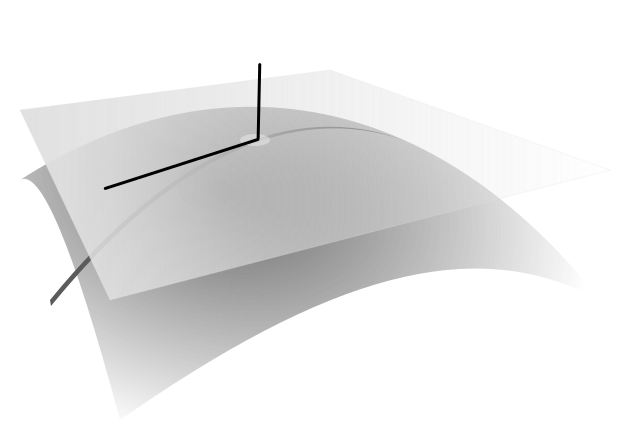
\includegraphics[width=0.8\textwidth]{tangent.pdf}
    \caption{Tangent plane and normal vector}
\end{figure}


\section{Derivatives of vector fields}

\begin{definition}[directional derivative]
    Let \(S\subset \bR^n\) and \(\ff:S\to \bR^m\).
    For any \(\aa \in \operatorname{int}S\) and \(\vv \in \bR^n\) the derivative of \(f\) with respect to \(\vv\) is defined as
    \[
        D_{\vv}\ff(\aa) :=
        \lim_{h\to 0} \frac{\ff(\aa+h \vv) - \ff(\aa)}{h}.
    \]
\end{definition}

Note: If we write \(\ff = (f_1,\ldots,f_m)\) then \(D_{\vv}\ff = (D_{\vv}f_1,\ldots,D_{\vv} f_m)\).


\begin{definition}[differentiable]
    We say that \(f\) is \emph{differentiable} at \(\aa\) if there is a linear transformation \(\mathbf{T}_\aa : \bR^n \to \bR^m\) and \(\mathbf{E}(\aa,\vv)\) such that, for \(\vv\in B(\aa,r)\),
    \[
        \ff(\aa+\vv) = \ff(\aa) + \mathbf{T}_\aa  (\vv )+ \norm{\vv}\mathbf{E}(\aa,\vv)
    \]
    and \(\mathbf{E}(\aa,\vv) \to 0\) as \(\vv \to 0\).
\end{definition}


\begin{theorem}
    If \(\ff\) is differentiable at \(\aa\)
    then \(\ff\) is continuous at \(\aa\)
    and \( \mathbf{T}_{\aa}( \vv) =D_{\vv}\ff(\aa) \).
\end{theorem}

\begin{proof}
    Same as for the case when \(f:\bR^n \to \bR\).
\end{proof}


\section{Jacobian matrix and chain rule}

In general, the relevant differential for higher-dimensional functions is the \href{https://en.wikipedia.org/wiki/Jacobian_matrix_and_determinant}{Jacobian matrix}.

\begin{definition}[Jacobian matrix]
    The \emph{Jacobian matrix} of \(\ff : \bR^n \to \bR^m\) at \(\aa\) is defined as
    \[
        D\ff(\aa) =
        \begin{pmatrix}
            \partial_1 f_1 (\aa) & \partial_2 f_1 (\aa) & \cdots & \partial_n f_1 (\aa) \\
            \partial_1 f_2 (\aa) & \partial_2 f_2 (\aa) & \cdots & \partial_n f_2 (\aa) \\
            \vdots               & \vdots               &        & \vdots               \\
            \partial_1 f_m (\aa) & \partial_2 f_m (\aa) & \cdots & \partial_n f_m (\aa)
        \end{pmatrix}
    \]

\end{definition}




\begin{itemize}
    \item Choosing a basis any linear transformation can be written as a \(m \times n\) matrix.
    \item \( \mathbf{T}_\aa  (\vv ) = D\ff(\aa) \vv\).
\end{itemize}

Let \(S\subset \bR^n\) and \(\ff : S \to \bR^m\).
If \(f\) is differentiable at \(\aa \in S\) then, for all  \(\vv\in B(\aa,r) \subset S\),
\[
    \ff(\aa+\vv) = \ff(\aa) +  D\ff(\aa) \vv + \norm{\vv}\mathbf{E}(\aa,\vv).
\]


This is like a Taylor expansion in higher dimensions.


Here we see that in higher dimensions we have a matrix form of the chain rule.

\begin{theorem}
    \label{thm:jacobian-chain}
    Let \(S\subset \bR^l\), \(T\subset \bR^m\) be open.
    Let \(\ff: S \to T\) and \(\gg:T \to \bR^n\) and define
    \[
        \hh := \gg \circ \ff : S \to \bR^n.
    \]
    Let  \(\aa\in S\). Suppose that \(\ff\) is differentiable at \(\aa\) and \(\gg\) is differentiable at \(\ff(\aa)\).
    Then \(\hh\) is differentiable at \(\aa\) and
    \[
        D\hh(\aa) = D\gg(\ff(\aa)) \ D\ff(\aa).
    \]
\end{theorem}

\vspace{-1em}

\begin{proof}
    Since \(\ff\) and \(\gg\) are differentiable there exists \(\mathbf{E}_{\ff}\) and \(\mathbf{E}_{\gg}\).
    Let \(\uu := \ff(\aa+\vv) - \ff(\aa) \).
    \[
        \begin{aligned}
            \hh(\aa+\vv) - \hh(\aa)
             & = \gg(\ff(\aa+\vv)) - \ff(\hh(\aa))                                                                                               \\
             & = D\gg(\ff(\aa))(\ff(\aa+\vv) - \ff(\aa) ) + \norm{\uu}\mathbf{E}_{\gg}(\ff(\aa),\uu)                                             \\
             & = D\gg(\ff(\aa))   D\ff(\aa) \vv + \norm{\vv}D\gg(\ff(\aa))\mathbf{E}_{\ff}(\aa, \vv) + \norm{\uu}\mathbf{E}_{\gg}(\ff(\aa),\uu).
        \end{aligned} \qedhere
    \]
\end{proof}



\begin{example}
    Here we consider \emph{polar coordinates} and calculate the Jacobian of this transformation.
    \begin{itemize}
        \item
              We can write the change of coordinates
              \((r,\theta) \mapsto (r\cos \theta, r\sin \theta)\)
              as the function  \(\ff(r,\theta) = (x(r,\theta),y(r,\theta))\) where \(\ff:(0,\infty)\times [0,2\pi) \to \bR^2\).
        \item
              We calculate the Jacobian matrix
              \[
                  D\ff(r,\theta) =
                  \begin{pmatrix}
                      \partial_{r}x(r,\theta) & \partial_{\theta}x(r,\theta) \\
                      \partial_{r}y(r,\theta) & \partial_{\theta}y(r,\theta)
                  \end{pmatrix}
                  =
                  \begin{pmatrix}
                      \cos \theta & -r\sin \theta \\
                      \sin \theta & r\cos \theta
                  \end{pmatrix}.
              \]
        \item
              We wish to calculate derivatives of \(h := g \circ \ff\) for some  \(g:\bR^2 \to \bR\).
              \[
                  \begin{aligned}
                      Dh(r,\theta) & = Dg(\ff(r,\theta)) \ D\ff(r,\theta) \\
                      \begin{pmatrix}
                          \partial_r h(r,\theta) & \partial_\theta h(r,\theta)
                      \end{pmatrix}
                                   & =
                      \begin{pmatrix}
                          \partial_x g(\ff(r,\theta)) & \partial_y g(\ff(r,\theta))
                      \end{pmatrix}
                      \begin{pmatrix}
                          \cos \theta & -r\sin \theta \\
                          \sin \theta & r\cos \theta
                      \end{pmatrix}
                  \end{aligned}
              \]

        \item Consequently
              \[
                  \begin{cases}
                      \partial_r h(r,\theta) = \partial_x g(r\cos \theta, r\sin \theta) \cos \theta + \partial_y g(r\cos \theta, r\sin \theta)\sin \theta \\
                      \partial_\theta h(r,\theta) = - r \partial_x g(r\cos \theta, r\sin \theta) \sin \theta +  r \partial_y g(r\cos \theta, r\sin \theta)\cos \theta
                  \end{cases}.
              \]
    \end{itemize}
\end{example}






\section{Implicit functions and partial derivatives}


We consider the following equality of partial derivatives.
Imagining the application of the partial derivative we can convince ourselves that it is something reasonable.

Does \(\partial_1\partial_2 f = \partial_2\partial_1 f\), etc.?

\begin{example*}[partial derivative problem]
    Let \(f:\bR^2 \to \bR\) be defined as \(f(0,0)=0\) and, for \((x_1,x_2)\neq (0,0)\),
    \[
        f(x_1,x_2) := \frac{x_1x_2(x_1^2 - x_2^2)}{x_1^2 + x_2^2}.
    \]
    We can calculate \(\partial_2\partial_1 f (0,0) = -1\) but
    \(\partial_1\partial_2 f(0,0) = 1\).
\end{example*}

\begin{theorem}
    Let \(f:S\to\bR\) be a scalar field such that the partial derivatives \(\partial_1 f\), \(\partial_2 f\) and \(\partial_2\partial_1 f\) exist on an open set \(S\subset \bR^2\) containing \(\xx\).
    Further assume that \(\partial_2\partial_1 f\) is continuous on \(S\).
    Then the derivative \(\partial_1\partial_2 f(\xx)\) exists and \(\partial_1\partial_2 f(\xx)=\partial_2\partial_1 f(\xx)\).
\end{theorem}

In many cases we can choose to write a given curve/function either in \emph{implicit} or \emph{explicit} form.

\begin{center}
    \begin{tabular}{c | c}
        \textbf{Implicit}     & \textbf{Explicit}                              \\
        \hline
        \(x^2-y=0\)           & \(y(x) = x^2\)                                 \\
        \(x^2+y^2-1=0\)       & \(y(x) = \pm \sqrt{1-x^2}\), \(\abs{x}\leq 1\) \\
        \(x^2-y^2-1=0\)       & \(y(x) = \pm \sqrt{x^2-1}\), \(\abs{x}\geq 1\) \\
        \(x^2+y^2-e^y -4 =0\) & A mess?
    \end{tabular}
\end{center}

Given the above observation, the following method of calculating derivatives is sometimes useful.
Suppose that some \(f:\bR^2 \to \bR\) is given and we suppose there exists some \(y:\bR\to\bR\) such that
\[
    f(x,y(x))=0 \quad \text{ for all \(x\)}.
\]
Let \(h(x):= f(x,y(x))\) and note that \(h'(x)=0\).
Here we are using the idea that \(h = f \circ g\) where \(g(x) = (x,y(x))\).
By the chain rule \( h'(x)\) is equal to
\[
    \begin{pmatrix}
        \frac{\partial f}{\partial x}(x,y(x)) & \frac{\partial f}{\partial y}(x,y(x))
    \end{pmatrix}
    \begin{pmatrix}
        1 \\
        y'(x)
    \end{pmatrix}
    =0.
\]
Consequently
\[
    y'(x) = - \frac{ \frac{\partial f}{\partial x}(x,y(x)) }{ \frac{\partial f}{\partial y}(x,y(x)) }.
\]
A similar argument also holds in higher dimension.


\section*{Worked examples}

\subsection*{Jacobian matrix}

\question
Let $\mathbf{f}:\mathbb{R}^2\to\mathbb{R}^2$, $\mathbf{g}:\mathbb{R}^3\to\mathbb{R}^2$ be defined as
\[
    \begin{aligned}
        \mathbf{f}(x,y) &= (e^{x+2y}, \sin(y+2x)) \\
        \mathbf{g}(u,v,w) &= (u+2v^2+3w^3,2v-u^2).
    \end{aligned}
\]
Let $\mathbf{h} =\mathbf{f} \circ \mathbf{g} : \bR^3 \to \bR^2$ and calculate \(D\mathbf{h}(1,-1,1)\).

\solution
We first calculate \(\mathbf{g}(1,-1,1) = (6,-3)\) and 
\[
    \begin{aligned}
        D\mathbf{f}(x,y) &= 
        \begin{pmatrix}
           e^{x+2y} & 2 e^{x+2y}\\
           2 \cos(y+2x) & \cos(y+2x)
        \end{pmatrix},\\
        D\mathbf{g}(u,v,w) &= 
        \begin{pmatrix}
            1 & 4v & 9w^2 \\
            -2u & 2 & 0
        \end{pmatrix}.   
    \end{aligned}
\]
Consequently
\[
    \begin{aligned}
        D\mathbf{f}(6,-3) &= 
        \begin{pmatrix}
           1 & 2 \\
           2 \cos 9 & \cos 9
        \end{pmatrix},\\
        D\mathbf{g}(1,-1,1) &= 
        \begin{pmatrix}
            1 & -4 & 9 \\
            -2 & 2 & 0
        \end{pmatrix}.   
    \end{aligned}
\]
By the chain rule for Jacobian matrices (Theorem~\ref{thm:jacobian-chain}),
\( D\mathbf{h}(1,-1,1) = D\mathbf{f}(6,-3)  D\mathbf{g}(1,-1,1) \)
and so, multiplying the matrices, we obtain 
$$D\mathbf{h}(1,-1,1) =
    \begin{pmatrix}
        -3 & 0 & 9 \\
        0        & -6\cos 9 & 18\cos 9
    \end{pmatrix}.
$$







\end{document}
